\documentclass{ctexbook}
\usepackage{xeCJK}
\usepackage{amsmath}
\usepackage{titlesec}
\usepackage{booktabs}
%\usepackage{tabularx}

\usepackage{enumitem}
\setlist{nolistsep}
\renewcommand\labelenumi{(\theenumi)}

\usepackage{scrextend}% not needed with a KOMA-Script class, provides the
                      % `addmargin' environment

\usepackage{exsheets}
\DeclareInstance{exsheets-heading}{mylist}{default}{
  runin = true ,
  attach = {
    main[l,vc]number[l,vc](-3em,0pt) ; % 3em = indent of question body
    main[r,vc]points[l,vc](\linewidth+\marginparsep,0pt)
  }
}
\SetupExSheets{
  headings = mylist , % use the new headings instance
  headings-format = \normalfont ,
  %counter-format = \thechapter.qu ,
  counter-within = section ,
  solution/print = true
}
\let\oldquestion\question
\let\oldsolution\solution

\renewenvironment{question}{%
	\SetupExSheets{counter-format=\thechapter.qu}
	\oldquestion
}

\renewenvironment{solution}{%
	\SetupExSheets{counter-format=}
	\oldsolution
}

\usepackage{etoolbox}
% 3em = indent of question body :
\AtBeginEnvironment{question}{\addmargin[3em]{0em}}
\AtEndEnvironment{question}{\endaddmargin}
\AtBeginEnvironment{solution}{\addmargin[3em]{0em}}
\AtEndEnvironment{solution}{\endaddmargin}

\title{人工智能及其应用(第4版)\\ 习题解析}
\date{}

\begin{document}
\maketitle

\chapter{绪论}

\begin{question}
什么是人工智能?试从学科和能力两方面加以说明。
\end{question}	
\begin{solution}
\end{solution}

\begin{question}
在人工智能的发展过程中,有哪些思想和思潮起了重要作用?
\end{question}
\begin{solution}
\end{solution}

\begin{question}
在过去的20年中,人工智能发生了什么变化?
\end{question}
\begin{solution}
\end{solution}

\begin{question}
为什么能够用机器(计算机)模仿人的智能?
\end{question}
\begin{solution}
\end{solution}

\begin{question}
现在人工智能有哪些学派?它们的认知观是什么?现在这些学派的关系如何?
\end{question}
\begin{solution}
\end{solution}

\begin{question}
你认为应从哪些层次对认知行为进行研究?
\end{question}
\begin{solution}
\end{solution}

\begin{question}
你是如何理解人工智能的研究目标的?
\end{question}
\begin{solution}
\end{solution}

\begin{question}
人工智能研究包括哪些内容?这些内容的重要性如何?
\end{question}
\begin{solution}
\end{solution}

\begin{question}
人工智能的基本研究方法有哪几类?它们与人工智能学派的关系如何?
\end{question}
\begin{solution}
\end{solution}

\begin{question}
人工智能的主要研究和应用领域是什么?其中,哪些是新的研究热点?
\end{question}
\begin{solution}
\end{solution}

\begin{question}
你对人工智能课程教学有何意见和建议?
\end{question}
\begin{solution}
\end{solution}
\chapter{知识表示方法}

\begin{question}
状态空间法、问题归约法、谓词逻辑法和语义网络法的要点是什么?它们有何本质上的联系及异同点?
\end{question}	
\begin{solution}
状态空间法:基于解答空间的问题表示和求解方法,它是以状态和算符为基础来表示和求解问题的。一般用状态空间法来表示下述方法:从某个初始状态开始,每次加一个操作符,递增的建立起操作符的试验序列,直到达到目标状态为止。 \par
问题规约法:已知问题的描述,通过一系列变换把此问题最终变成一个子问题集合:这些子问题的解可以直接得到,从而解决了初始问题。问题规约的实质:从目标(要解决的问题)出发逆向推理,建立子问题以及子问题的子问题,直至最后把出示问题规约为一个平凡的本原问题集合。状态空间法是问题归约法的一种特例。在问题归约法的与或图中,包含有与节点和或节点,而在状态空间法中只含有或节点。 \par
谓词逻辑法:采用谓词合式公式和一阶谓词算法。要解决的问题变为一个有待证明的问题,然后采用消解定理和消解反演莱证明一个新语句是从已知的正确语句导出的,从而证明这个新语句也是正确的。\par
语义网络法:是一种结构化表示方法,它由节点和弧线或链组成。节点用于表示物体、概念和状态,弧线用于表示节点间的关系。语义网络的解答是一个经过推理和匹配而得到的具有明确结果的新的语义网络。语义网络可用于表示多元关系,扩展后可以表示更复杂的问题。语义网络法与谓词逻辑法等效。\par
它们的本质都是对一具体事实知识表示,只是表示的方法不同。对于同一问题可以有许多不同的表示方法。不过对于特定问题,有的表示方法比较有效,其他表示方法可能不大适用,或者不是好的表示方法。在表示和求解比较复杂的问题时,采用单一的知识表示方法是远远不够的,往往必须采用多种方法混合表示。此外,在选择知识表示方法时,还要考虑所使用的程序设计语言所提供的功能和特点,以便能够更好地描述这些表示方法。
\end{solution}

\begin{question}
设有$3$个传教士和$3$个野人来到河边,打算成一条船从右岸渡到左岸去。该船的负载能力为两人。在任何时候,如果野人人数超过传教士人数,那么野人就会把传教士吃掉。怎样才能用这条船安全地把所有人都渡过河去?
\end{question}
\begin{solution}
设$(m,n)$表示右岸上有$m$个野人,$n$个传教士;$r(m,n)$表示把$m$个野人和$n$个传教士从右岸运至左岸,$l(m,n)$表示把$m$个野人和$n$个传教士从左岸运至右岸。则安全把所有人渡过河的过程表示为
\begin{align*}
& (3,3) \xrightarrow{r(2,0)} (1,3) \xrightarrow{l(1,0)} (2,3) 
	\xrightarrow{r(2,0)} (0,3) \xrightarrow{l(1,0)} (1,3) \\
	\xrightarrow{r(0,2)} & (1,1) \xrightarrow{l(1,1)} (2,2) 
	\xrightarrow{r(0,2)} (2,0) \xrightarrow{l(1,0)} (0,0) \xrightarrow{r(2,0)} (0,0)
\end{align*}
\end{solution}

\begin{question}
利用图\ref{Fig:TSP-problem},用状态空间法规划一个最短的旅行路程:此旅程从城市A开始,访问其他城市不多于一次,并返回A。选择一个状态表示,表示出所求得的状态空间的节点及弧线,标出适当的代价,并指明图中从起始节点到目标节点的最佳路径。
\begin{figure} [h]
		\centering
		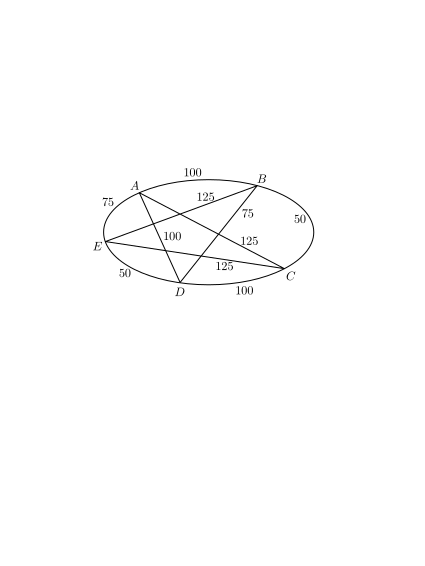
\includegraphics[scale=.8]{figures/ques-2.3.pdf}
		\caption{旅行商问题} \label{Fig:TSP-problem}
	\end{figure}
\end{question}
\begin{solution}
用状态空间法表示所求路径如图\ref{Fig:TSP-answer}所示。
	\begin{figure} [h]
		\centering
				\begin{forest}
		  for tree={
		    draw,
		    circle,
		  },
		  [A
		  	[B, edge label={node[midway,left,font=\scriptsize]{100}}
		  		[C, edge label={node[midway,left,font=\scriptsize]{150}}
		  			[D, edge label={node[midway,left,font=\scriptsize]{100}}
		  				[E, edge label={node[midway,right,font=\scriptsize]{50}}
		  					[A, edge label={node[midway,right,font=\scriptsize]{75}}
		  					]]]
		  			[E, edge label={node[midway,right,font=\scriptsize]{125}}
		  				[D, edge label={node[midway,right,font=\scriptsize]{50}}
		  					[A, edge label={node[midway,right,font=\scriptsize]{100}}
		  					]]]
		  		][D, edge label={node[midway,right,font=\scriptsize]{75	}}
		  			[C, edge label={node[midway,left,font=\scriptsize]{100}}
		  				[E, edge label={node[midway,right,font=\scriptsize]{125}}
		  					[A, edge label={node[midway,right,font=\scriptsize]{75}}
		  					]]]
		  			[E, edge label={node[midway,right,font=\scriptsize]{50}}
		  				[C, edge label={node[midway,right,font=\scriptsize]{125}}
		  					[A, edge label={node[midway,right,font=\scriptsize]{125}}
		  					]]]
		  		][E, edge label={node[midway,right,font=\scriptsize]{125}}
					[C, edge label={node[midway,left,font=\scriptsize]{125}}
						[D, edge label={node[midway,right,font=\scriptsize]{100}}
							[A, edge label={node[midway,right,font=\scriptsize]{100}}
							]]]
					[D, edge label={node[midway,right,font=\scriptsize]{50}}
						[C, edge label={node[midway,right,font=\scriptsize]{100}}
							[A, edge label={node[midway,right,font=\scriptsize]{125}}
							]]]  		
		  		]
		  	][C][D][E]
		  ]
		\end{forest}
		\caption{旅行商问题状态空间图} \label{Fig:TSP-answer}
	\end{figure}
\end{solution}

\begin{question}
试说明怎样用一棵与或解树来表达图\ref{Fig:elec}所示的电网络阻抗的计算。单独的$R$、$L$或$C$可分别用$R$、$j\omega L$或$1/j\omega C$来计算,这个事实用作本原问题。后继算符应以复合并联和串联阻抗的规则为基础。
	\begin{figure}[H]
		\centering
		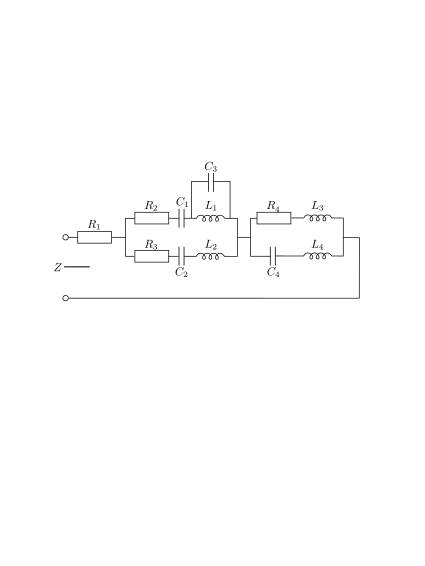
\includegraphics{figures/ques-2.4.pdf}
		\caption{电网络阻抗计算} \label{Fig:elec}
	\end{figure}
\end{question}
\begin{solution}
约定,用原来的与后继算法用来表达并联关系,用原来的或后继算法用来表达串联关系。则所求与或解树如图\ref{Fig:and-or-tree-for-elec}所示。
\end{solution}

	\begin{figure}[H]
		\centering
		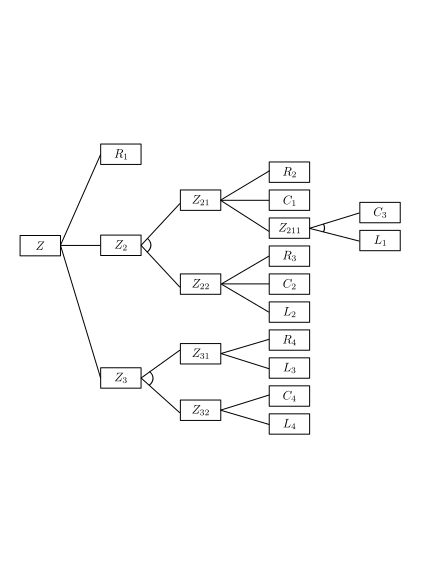
\includegraphics[scale=.8]{figures/ans-2.4.pdf}
		\caption{电网络阻抗计算与或解树} \label{Fig:and-or-tree-for-elec}
	\end{figure}

	\begin{figure}[H]
		\centering
		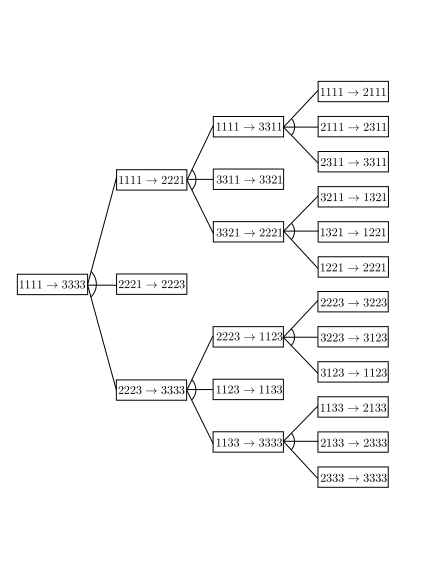
\includegraphics[scale=.8]{figures/ans-2.5.pdf}
		\caption{樊塔问题与或树} \label{Fig:and-or-tree-for-hannoi}
	\end{figure} 

\begin{question}
试用四元数列结构表示四圆盘梵塔问题,并画出求解该问题的与或图。
\end{question}
\begin{solution}
用四元数列$(n_A, n_B, n_C, n_D)$来表示A、B、C、D盘分别落在$n_A$、$n_B$、$n_C$、$n_D$号柱子上。则问题的初始状态为$(1,1,1,1)$,目标状态为$(3,3,3,3)$。\par
求解问题的与或图如图\ref{Fig:and-or-tree-for-hannoi},按从上往下的顺序,依次处理每一个叶结点,搬动圆盘,问题得解。
\end{solution}

\begin{question}
把下列句子变换成子句形式:
	\begin{enumerate}
         \item $\left(\forall x\right) \left\{P\left(x\right) \to P\left(x\right)\right\}$
         \item $\forall x \forall y \left(\mathrm{On} \left(x,y\right) \to \mathrm{Above} \left(x,y\right) \right)$
         \item $\forall x \forall y \forall z \left(\mathrm{Above} \left(x,y\right) \wedge \mathrm{Above}\left(y,z\right) \to \mathrm{Above}\left(x,z\right) \right)$ 
         \item $\sim\left\{\left(\forall x\right)\left\{\left(\forall y)\left[p\left(y\right) \to p(f(x,y))\right] \wedge \left(\forall y \right) \left[Q(x,y) \to P(y) \right]\right\}\right\}\right\}$
	\end{enumerate}
\end{question}
\begin{solution}
	\begin{enumerate}
		 \item $\left(\forall x\right) \left\{P\left(x\right) \to P\left(x\right)\right\}$ \\
		 	消去蕴含符号:
		 	\[(\forall x) [ \sim P(x) \vee P(x)] \]
		 	消去全称量词:
		 	\[\sim P(x) \vee P(x) \]
		 	得到句子:
		 	\[\sim P(x) \vee P(x) \]
		 	
         \item $\forall x \forall y \left(\mathrm{On} \left(x,y\right) \to \mathrm{Above} \left(x,y\right) \right)$ \\
         	消去蕴含符号:
         	\[ \forall x \forall y [\sim \mathrm{On} (x,y) \vee \mathrm{Above} (x,y)] \]
         	消去全称量词:
         	\[ \sim \mathrm{On} (x,y) \vee \mathrm{Above} (x,y) \]
         	得到句子:
         	\[ \sim \mathrm{On} (x,y) \vee \mathrm{Above} (x,y) \]
         \item $\forall x \forall y \forall z \left(\mathrm{Above} \left(x,y\right) \wedge \mathrm{Above}\left(y,z\right) \to \mathrm{Above}\left(x,z\right) \right)$ \\
         	消去蕴含符号:
         	\[ \forall x \forall y \forall z \{ \sim [ \mathrm{Above} (x,y) \wedge \mathrm{Above} (y,z) \wedge \mathrm{Above} (x,z) \} \]
         	消去全称量词:
         	\[ \sim [ \mathrm{Above} (x,y) \wedge \mathrm{Above} (y,z) ] \vee \mathrm{Above} (x,z)\]
         	得到句子:
         	\[ \sim \mathrm{Above} (x,y) \vee \sim \mathrm{Above(x,z)} \vee \mathrm{Above} (y,z) \]
         	
         \item $\sim\left\{\left(\forall x\right)\left\{\left(\forall y)\left[p\left(y\right) \to p(f(x,y))\right] \wedge \left(\forall y \right) \left[Q(x,y) \to P(y) \right]\right\}\right\}\right\}$ \\
         	消去蕴含符号:
         	\begin{multline*}
         	\sim \left\{ (\forall x) \left\{ \sim P(x) \vee \right. \right. \\
         	\left. \left. \left\{ (\forall y) \left[ \sim p(y) \vee p \left( f(x,y) \right) \right] \wedge (\forall y) \left[ \sim Q(x,y) \vee P(y) \right] \right\} \right\} \right\} 
         	\end{multline*}
         	减少否定符号的辖域:
         	\begin{multline*}
         	(\exists x) \left\{ P(x) \wedge \right. \\
         	\left. \left\{ (\exists x) \left[ p(y) \wedge \sim p \left( f(x,y) \right) \right] \vee (\exists y) \left[ Q(x,y) \wedge \sim P(y) \right] \right\} \right\} 
         	\end{multline*}
         	对变量标准化:
         	\begin{multline*} 
         	(\exists x) \left\{ P(x) \wedge \right. \\
         	\left. \left\{ (\exists w) \left[ p(y) \wedge \sim p \left( f(w,y) \right) \right] \vee (\exists v) \left[ Q(x,v) \wedge \sim P(v) \right] \right\} \right\} 
         	\end{multline*}
         	消去存在量词:
         	\[ P(A) \wedge \left\{ \left[ p(y) \wedge \sim p \left( f(B,y) \right) \right] \vee \left[ Q(A,C)\wedge \sim P(C)  \right] \right\} \]
         	把母式化为合取范式:
         	\begin{multline*}
         	P(A) \wedge \left\{ \left[ p(y) \wedge \sim p \left( f(B,y) \right) \vee Q(A,C) \right] \wedge \right. \\
         	\left. \left[ p(y) \wedge \sim p\left( f(B,y) \right) \vee \sim P(C) \right] \right\} 
         	\end{multline*}
         	消去连词符号(合取):
         	\begin{multline*}
         	P(A) \wedge \left\{ \left[ p(y) , \sim p \left( f(B,y) \right) \right] \vee Q(A,C) \right\} \wedge \\
         	\left\{ \left[ p(y) , \sim p\left( f(B,y) \right) \right] \vee \sim P(C) \right\}
         	\end{multline*}
         	得到子句:
         	\begin{align*}
         	& P(A) \\
         	& \left[ p(y) , \sim p \left( f(B,y) \right) \right] \vee Q(A,C)  \\
         	& \left[ p(y) , \sim p\left( f(B,y) \right) \right] \vee \sim P(C)
         	\end{align*}
	\end{enumerate}
\end{solution}

\begin{question}
用谓词演算公式表示下列英文句子(多用而不是省用不同谓词和项。例如不要用单一的谓词字母来表示每个句子)。
	\begin{quote}
		A computer system is intelligent if it can perform a task which, if performed by a human, requires intelligence. 
	\end{quote}
\end{question}
\begin{solution}
定义以下谓词:
	\begin{itemize}
		\item $\mathrm{INTLT}(x)$:	$x$ is intelligent.
		\item $\mathrm{PERFORM}(x,y)$:	$x$ can perform $y$.
		\item $\mathrm{REQUIRE}(x)$:		$x$ requires intelligence.
		\item $\mathrm{CMP}(x)$:		$x$ is a computer system.
		\item $\mathrm{HMN}(x)$:		$x$ is a human.
	\end{itemize} \par
则题中句子可以表达为
	\begin{multline*}
	\left( \exists t \right) \left( \exists y \right)
	\left[ \mathrm{HMN}(x) \vee \mathrm{PERFORM}(y,t) \vee \mathrm{REQUIRE}(t)
	\vee \mathrm{CMP}(x) \right. \\
	\left. \vee \mathrm{PERFORM}(x,t) \right] 
	\to \mathrm{INTLT}(x)
	\end{multline*}
\end{solution}

\begin{question}
把下列语句表示称语义网络描述:
	\begin{enumerate}
		\item All men are moral.
		\item Every cloud has a silver lining.
		\item All branch manager of DEC participate in a profit-sharing plan. 
	\end{enumerate}
\end{question}
\begin{solution}
如图\ref{Fig:semantic-net}。
	\begin{figure}[h]
		\centering
		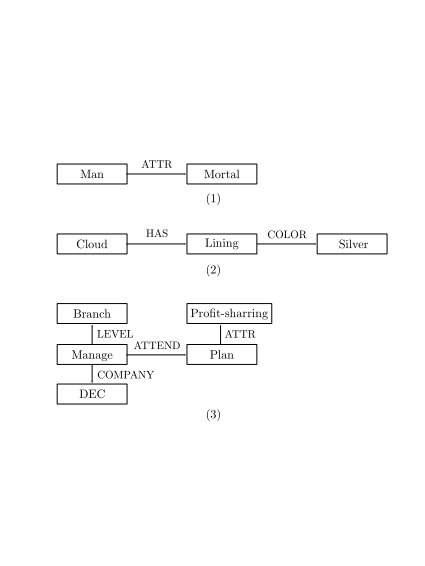
\includegraphics[scale=.9]{figures/ans-2.8.pdf}
		\caption{ 所求语义网络 } \label{Fig:semantic-net}
	\end{figure}
\end{solution}

\begin{question}
试构造一个描述你的寝室或办公室的框架系统。
\end{question}
\begin{solution}
以房间为例,如图\ref{Fig:semantic-my-room}。
	\begin{figure}[h]
		\centering
		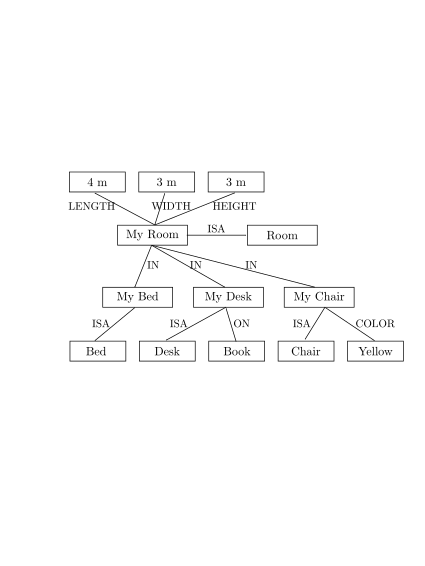
\includegraphics[scale=.9]{figures/ans-2.9.pdf}
		\caption{ 我的房间语义网络 } \label{Fig:semantic-my-room}
	\end{figure}
\end{solution}

\begin{question}
框架和本体有何关系与区别?
\end{question}
\begin{solution}
框架是一种结构化表示方法。框架通常由指定事物各个方面的槽组成,每个槽拥有若干个侧面,而每个侧面又可拥有若干个值。大多数实用系统必须同时使用许多框架,并可把它们联成一个框架系统。框架表示已获广泛应用,然而并非所有问题都可以用框架表示。\par
本体是概念化的一个显示规范说明或表示。本体可定义为被共享的概念化的一个形式规范说明。本体是一种比框架更有效的表示方法。
\end{solution}
\chapter{确定性推理}

\begin{question}
什么是图搜索过程?其中,重排OPEN表意味着什么?重排的原则是什么?
\end{question}	
\begin{solution}
图搜索的一般过程如下:
	\begin{enumerate}
		\item 建立一个只含有起始节点$S$的搜索图$G$,把S放到一个叫做OPEN的未扩展节点表中。
		\item 建立一个叫CLOSED的已扩展节点表,其初始为空表。
		\item LOOP:检查OPEN表是否为空,若为空,则失败退出。
		\item 选择OPEN表上的第一个节点,把它从$OPEN$表移出放进$CLOSED$表。并记该节点为节点$n$。
		\item 考察节点$n$是否为目标节点。若$n$为一目标节点,则有解并成功退出。此解是追踪图$G$中沿着指针从$n$到$S$这条路径而得到的(指针将在第7步中设置)。
		\item 扩展节点$n$,生成一组子节点。把这些子节点中不是$n$的祖先的那些后继节点记入集合$M$。把M的这些成员作为$n$的后继节点添入图$G$中。
		\item 针对M中子节点的不同情况,分别作如下处理:
			\begin{itemize}
				\item 未曾在$G$中出现过的$M$成员设置一个通向其父节点(即节点$n$)的指针,并把M的这些成员加进OPEN表。(新生成的)
				\item 对已经在OPEN或CLOSED表上的每一个$M$成员,确定是否需要更改通到其父节点$n$的指针方向。(原生成但未扩展的)
				\item 对已在CLOSED表上的每个$M$成员,确定是否需要更改图$G$中通向它的每个后裔节点的指针方向。(原生成也扩展过的)
			\end{itemize}
		\item 按某一任意方式或按某个探试值,重排OPEN表。
		\item GO LOOP。
	\end{enumerate} \par
重排OPEN表意味着什么, 在第(6)步中,将优先扩展哪个节点,不同的排序标准对应着不同的搜索策略。是否重新安排OPEN表,即是否按照某个试探值(或准则、启发信息等)重新对未扩展节点进行排序,将决定该图搜索过程是无信息搜索或启发式搜索。各种搜索策略的主要区别在于对OPEN表中节点的排列顺序不同。例如,广度优先搜索把先生成的子节点排在前面,而深度优先搜索则把后生成的子节点排在前面。\par
重排的原则当视具体需求而定,不同的原则对应着不同的搜索策略,如果想尽快地找到一个解,则应当将最有可能达到目标节点的那些节点排在OPEN表的前面部分,如果想找到代价最小的解,则应当按代价从小到大的顺序重排OPEN表。
\end{solution}

\begin{question}
试举例比较各种搜索方法的效率。
\end{question}	
\begin{solution}
	\begin{description}
		\item[宽度优先搜索] 只要问题有解,用宽度优先搜索总可以得到解,而且得到的是路径最短的解。宽度优先搜索盲目性较大,当目标节点距初始节点较远时将会产生许多无用节点,搜索效率低。
		\item[深度优先搜索] 搜索一旦进入某个分支,就将沿着该分支一直向下搜索。如果目标节点恰好在此分支上,则可较快地得到解。但是,如果目标节点不在此分支上,而该分支又是一个无穷分支,则就不可能得到解。所以深度优先搜索是不完备的,即使问题有解,它也不一定能求得解。所求得的解答路径不一定是最短路径。
		\item[有界深度优先搜索] 如果问题有解,且其路径长度$\leq dm$,则搜索过程一定能求得解。但是,若解的路径长度$> dm$,则搜索过程就得不到解。这说明在有界深度优先搜索中,深度界限的选择是很重要的。要恰当地给出$dm$的值是比较困难的。即使能求出解,它也不一定是最优解。
		\item[等代价搜索] 是宽度优先搜索的一种推广,不是沿着等长度路径断层进行扩展,而是沿着等代价路径断层进行扩展。搜索树中每条连接弧线上的有关代价,表示时间、距离等花费。若所有连接弧线具有相等代价,则简化为宽度优先搜索算法。
		\item[盲目搜索] 具有较大的盲目性,产生的无用节点较多,效率不高,耗费过多的计算空间与时间。
		\item[有序搜索] 利用启发信息,决定哪个是下一步要扩展的节点。选``最有希望''的节点作为下一个被扩展的节点。选择OPEN表上具有最小$f$值的节点作为下一个要扩展的节点, 又称为最佳优先搜索。正确选择估价函数对搜索结果具有决定性的作用。使用不能识别某些节点真实希望的估价函数会形成非最小代价路径;使用一个过多地估计了全部节点希望的估价函数又会扩展过多的节点。 
		\item[A算法] 虽提高了算法效率,但不能保证找到最优解。
		\item[A*算法] 搜索效率很大程度上取决于估价函数$h(n)$。一般来说,在满足$h(n)\leq h*(n)$的前提下,$h(n)$的值越大越好。$h(n)$的值越大,说明它携带的启发性信息越多,A*算法搜索时扩展的节点就越少,搜索效率就越高。
	\end{description}

\end{solution}

\begin{question}
化为子句型有哪些步骤?请结合例子说明。
\end{question}	
\begin{solution}
\end{solution}

\begin{question}
如何通过消解反演求取问题的答案。
\end{question}	
\begin{solution}
\end{solution}

\begin{question}
什么叫合式公式?合式公式有哪些等价关系?
\end{question}	
\begin{solution}
\end{solution}

\begin{question}
用宽度优先搜索求××所示迷宫的出路。
\end{question}
\begin{solution}
\end{solution}

\begin{question}
用有界深度优先搜索方法求解××所示八数码难题。
\end{question}
\begin{solution}
\end{solution}

\begin{question}
应用最新的方法表达传教士和野人问题,编写一个计算机程序,以求得安全渡过全部6个人的解答。(提示:在应用状态空间表示和搜索方法时,可用$(N_m,N_c)$来表示状态描述,其中$N_m$和$N_c$分别为传教士和野人的人数。初始状态为(3,3),而可能的中间状态为(0,1),(0,2),(0,3),(1,1),(2,1),(2,2),(3,0),(3,1)和(3,2)等。
\end{question}
\begin{solution}
\end{solution}

\begin{question}
试比较宽度优先搜索、有界深度优先搜索及有序搜索的搜索效率,并以实例数据加以说明。
\end{question}
\begin{solution}
\end{solution}

\begin{question}
一个机器人驾驶卡车,携带包裹(编号分别为\#1、\#2和\#3)分别投递到林(LIN)、吴(WU)和胡(HU) 3家住宅处。规定了某些简单的操作符,如表示驾驶方位的drive($x$,$y$)和表示卸下包裹的unload($z$);对于每个操作符,都有一定的先决条件和结果。试说明状态空间问题求解系统如何能够应用谓词演算求得一个操作符序列,该序列能够生成一个满足$\mathrm{AT(\# 1,LIN) \wedge AT(\# 2,WU) \wedge AT(\# 3,HU)}$的目标状态。
\end{question}
\begin{solution}
\end{solution}

\begin{question}
规则演绎系统和产生式系统有哪几种推理方式?各自的特点为是什么?
\end{question}
\begin{solution}
\end{solution}

\begin{question}
单调推理有何局限性?什么叫缺省推理?非单调推理系统如何证实一个节点的有效性?
\end{question}
\begin{solution}
单调系统不能很好地处理常常出现在现实问题领域中的3类情况,即不完全的信息、不断变化的情况、以及求解复杂问题过程中生成的假设。有两种方法可以证实节点的有效性:
	\begin{enumerate}
		\item 支持表。(SL (IN-节点表) (OUT-节点表)) \\
			如果某节点的IN节点表中提到的节点当前都是IN, 且OUT节点表中提到的节点当前都是OUT,则它是有效的。
		\item 条件证明。(CP(结论) (IN-假设) (OUT-假设)) \\
			条件证明(CP)的证实表示有前提的论点,无论何时,只要在IN假设中的节点为IN,OUT假设中的节点为OUT,则结论节点往往为IN,于是条件证明的证实有效。 
	\end{enumerate}
\end{solution}

\begin{question}
在什么情况下需要采用不确定推理或非单调推理?
\end{question}
\begin{solution}
不完全的信息、不断变化的情况、以及求解复杂问题过程中生成的假设。
\end{solution}

\begin{question}
下列语句是一些几何定理,把这些语句表示为基于规则的几何证明系统的产生式规则:
	\begin{enumerate}
		\item 两个全等三角形的各对应角相等。
		\item 两个全等三角形的各对应边相等。 
		\item 各对应边相等的三角形是全等三角形。
		\item 等腰三角形的两底角相等。 
	\end{enumerate}
\end{question}
\begin{solution}
	\begin{enumerate}
		\item IF 两个三角形全等 THEN 各对应角相等 
		\item IF 两个三角形全等 THEN 各对应边相等 
		\item IF 两个三角形各对应边相等 THEN 两三角形全等 
		\item IF 它是等腰三角形 THEN 它的两底角相等
	\end{enumerate}

\end{solution}

\end{document}